
% スタイルファイルの指定
% パッケージを使用する場合,ここで全て指定する.
\documentstyle[cite,a4j,twoside,12pt,enumerate,graphicx,listings,amssymb,subcaption,amsmath]{jbmdthesis}
% \documentclass[cite,a4j,twoside,12pt,enumerate,graphicx,listings,amssymb,subcaption,amsmath]{jbmdthesis}

% \usepackage[dvipdfmx]{graphicx}

% ヘッダを追加する
\pagestyle{headings}

% 画像元のパスの追加
\graphicspath{{figure/}}

\begin{document}

% 図,表,節などを参照するためのコマンドを定義
% これらのコマンドの使い方は template/ 内の Readme.md を参照すること
\newcommand{\fig}[1]{{図~\ref{fig:#1}}}
\newcommand{\subfig}[2]{{図~\ref{fig:#1}}~{(\subref{fig:#2})}}
\newcommand{\tab}[1]{{表~\ref{tab:#1}}}
\newcommand{\refchap}[1]{第{\ref{sec:#1}~章}}
\newcommand{\refsec}[1]{{\ref{sec:#1}~節}}
\newcommand{\ctext}[1]{\textcircled{\scriptsize{#1}}}

% ページ番号をアラビア数字にする(0,1,2,..)
\pagenumbering{roman}


% ---------- ユーザ入力ここから ----------
% タイトルページの情報
\title{\bf 容量効率を意識したソース・タグ値に \\
基づくセグメント化による\\
発行キューの電力削減}
\author{\bf 森 健一郎}
\date{3} % 令和~年

% 表紙を出力(自分の所属に応じてコメントを外す)
\minfotitle   % 修論
% \belectitle   % 卒論
% ---------- ユーザ入力ここまで ----------



% 概要を出力
{ 
  % 目次に影響がでないように, 
  % setlength のスコープを abstract 内だけに限定するためのブロック

  % 行間の調整
  \setlength{\baselineskip}{2.2em}
  
\chapter*{概要}
\markboth{概要}{概要}
発行キューは電力密度の大きいホット・スポットとして知られている.ホット・スポットは,デバイスの摩耗故障を引き起こし,誤動作やタイミング・エラーを引き起こす.発行キューが大きな電力を消費する原因は,ウェイクアップ論理のタグ比較回路である.この回路はCAMで構成されており,全てのデスティネーション・タグと発行キュー内の全てのソース・タグとの多数の比較を一斉に行うため,非常に大きな電力を消費する.そこで本論文では,CAM の分野で提案されている手法を応用し,タグ比較による消費電力を削減する手法を提案する.本手法では,発行キューを複数のセグメントに分割する.命令は,ソース・タグの下位ビットがセグメント番号と一致するセグメントにディスパッチする.そして,ウェイクアップ時には,ディスティネーション・タグの下位ビットが一致するセグメントにあるタグ比較器のみを動作させる.一致しないセグメントの比較器は動作しないため,タグ比較器の動作回数を削減できる.

本手法では,命令がディスパッチされるセグメントに空きがない場合,他のセグメントに空きがあってもディスパッチできないためストールする.この結果,発行キューの容量効率が低下するという問題が生じる.この問題は,発行キューの容量効率が重要なプログラムにおいて性能低下を引き起こす.そこで本論文では,容量効率を重視したディスパッチ・アルゴリズムと,タグ比較の積極的な削減を重視したディスパッチ・アルゴリズムを動的に切り替える手法を提案する.本手法は,発行キューの容量効率が重要な場合は容量効率の低下による性能低下を抑制し,そうでない場合は積極的にタグ比較器の動作回数を削減することを可能とする.提案手法を SPEC CPU 2017 を用いて評価を行った.結果,性能低下を最大で 5\% 以下(平均 -1\%)に抑えつつ,タグ比較器の動作回数を平均で 85\% 削減できることを確認した.

}

% 目次を出力
\tableofcontents

% ページ番号のリセット
\clearpage 
\pagenumbering{arabic}

% 行間の調整(これ以降ずっとこの行間)
\setlength{\baselineskip}{2.2em}



% ---------- ユーザ入力ここから ----------
% 各章の記述

\chapter{はじめに}
\label{sec:introduction}
現在のプロセッサは,非常に微細な LSI 技術で製造される.このような LSI の微細化に伴い,デバイスの信頼性低下の問題が深刻になっている~\cite{Weste2010}.微細化は,経年劣化や摩耗故障を加速し,その結果,タイミング・エラーや誤動作を引き起こし,デバイスの寿命を縮める.経年劣化や摩耗故障は温度に関して指数関数的に加速し~\cite{Monsieur2001,Khan2010,Black1969},温度10〜15℃の上昇でデバイスの寿命は半分以下になる~\cite{Viswanath2000}.

プロセッサ・チップ上には,ホット・スポットと呼ばれる単位面積あたりの電力が大きい場所が存在する.ホット・スポットは,そうでない場所と比べて温度上昇が激しいため,上述した故障を引き起こす確率が高くなる.従って,ホット・スポットを生成する回路の消費電力を低下させる必要がある.

ホット・スポットを生成する回路の1つに,発行キューがある.発行キューのサイズはプロセッサの世代が進むごとに大きくなっており,より深刻なホット・スポットとなっている.従って,発行キューの電力削減に対する要求は非常に大きい.
  
発行キューの中で最も電力を消費する回路は,タグ比較の回路である.タグ比較は,発行幅分のディスティネーション・タグとすべてのソース・タグとの間で行われるため,非常に多くの電力を消費する.そこで本論文では,タグ比較器が動作する回数を削減する以下のような手法を提案する.
\begin{itemize}
  \item 発行キューを複数の\textbf{セグメント}に分割する.命令を発行キューにディスパッチする際,第 1 ソース・タグの下位ビットが $n$ である命令は,第 $n$ 番目のセグメントに書き込む.タグ比較時には,ディスティネーション・タグの下位ビットがセグメント番号と一致するセグメントでのみ,第 1 ソース・タグの比較を行う.一致しないセグメントでは比較が行われない.これによりタグ比較回数が削減される.
  \item 上記の方法では,第 2 ソース・タグの比較回数は削減されない.そこで提案手法では\textbf{スワップ}と\textbf{サブ・セグメント}と呼ぶ 2 つの方法を導入し,第 2 ソース・タグの比較回数も削減する.スワップは,ディスパッチ時に第 1 ソース・オペランドがレディで,第 2 ソース・オペランドがレディでない命令において,第 1 ソース・タグと第 2  ソース・タグを格納するフィールドを交換し,第 2 ソース・タグの下位ビットを用いてディスパッチするセグメントを決定する手法である.サブ・セグメントは,各セグメントを第 2 ソース・タグにもとづきさらに分割する手法である.
  \item セグメント化によりディスパッチできるエントリが制限されるため,発行キューの容量効率が低下し,容量に敏感なプログラムにおいて性能が低下するという問題が存在する.この問題に対応するため,本論文では \textbf{SWITCH} という手法を提案する.SWITCH では,容量効率を重視したディスパッチ・アルゴリズムと,タグ比較回数の削減を重視したディスパッチ・アルゴリズムを,容量効率の重要性に応じて切り替えて使用することにより,性能低下を抑制する.
\end{itemize}

提案手法を SPEC CPU 2017 ベンチマークを用いて評価し,性能低下を 最大でも 5\% 以下(平均 -1\%)に抑えつつ,タグ比較の回数を平均で 85\% 削減できることを確認した.

本論文の残りの構成は次の通りである.まず,\ref{sec:issue_queue}節で発行キューの基本的な事項を説明する.そして,\ref{sec:segmented_IQ}節で提案手法の基本となるアイデアに関して説明した後,\ref{sec:second_tag_comp}節で提案手法における第 2  ソース・タグのタグ比較回数削減方法に関して述べる.その後,\ref{sec:occupency_reduction}節で提案手法の問題点である発行キューの容量効率の低下に関して説明した後,\ref{sec:switch}節で容量効率の低下に対する対策方法を説明する.\ref{sec:eval}節で評価を行い,\ref{sec:summary}節でまとめる.


% 本論文の構成は次の通りである.まず,\refchap{related_work}で関連研究を示す.\refchap{miss_assumed_pipeline}では MAP について説明する.その後,\refchap{hybrid_arc}で従来の構成と MAP を組み合わせたアーキテクチャについて述べ,\refchap{sw_algorithm}では提案するパイプラインの切り替えアルゴリズムについて述べる.\refchap{evaluation}では提案手法の評価を行い,最後に\refchap{summary}でまとめる.



\chapter{発行キュー(IQ:Issue Queue)}
\label{sec:basic_IQ}
本章では,本研究の研究対象である、IQ に関して説明する.まず,IQ の概要と動作を\refsec{iq_abst}で説明したあと,IQ の回路構成を\refsec{iq_circuit}で述べる.その後,\refsec{iq_scheme}でIQ の方式に関して説明する.

\section{概要と動作}
\label{sec:iq_abst}
IQ はアウト・オブ・オーダ実行を行うプロセッサにおいて,リネームされた命令を保持し,実行順序をスケジューリングして,機能ユニットへ発行する回路である.IQ は,ディスパッチ,発行,ウェイクアップと呼ばれる 3 種類の動作を行う.以下でそれぞれの動作に関して説明する.

\begin{itemize}
  \item ディスパッチ:リネームされた命令は,IQ にエントリが割り当てられ,命令の情報が格納される.この動作をディスパッチと呼ぶ.ディスパッチの動作は,IQ の方式により異なる.IQ の方式に関しては,\refsec{iq_scheme}で詳しく説明する.
  \item 発行:IQ 内の命令のうち,ソース・オペランドが両方共レディとなった命令は,依存関係が解消し,実行が可能となる.このような命令を実行ユニットに送出する動作を発行と呼ぶ.なお,発行可能な命令が機能ユニットの数を超える場合は,各命令の発行優先度に基づき命令を選択して発行する.発行された命令のエントリは IQ より削除される. 
  \item ウェイクアップ:命令が発行されると,その命令のディスティネーション・オペランドのタグと IQ 内にある全命令のソース・オペランドのタグの比較が行われる.比較が一致した場合には,対応するソース・オペランドのレディ・ビットをセットする.この動作をウェイクアップと呼ぶ.両方のオペランドがレディとなった命令は,依存が解消したため発行可能となる.
\end{itemize}

\begin{figure}[thb]
  \centering
  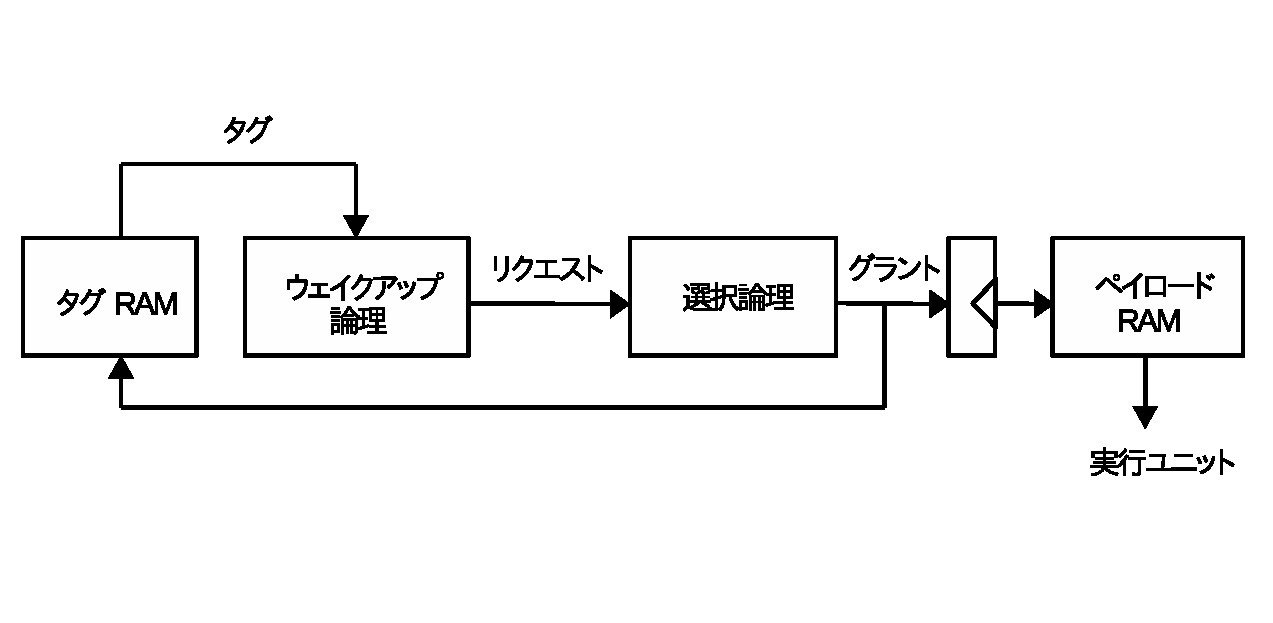
\includegraphics[keepaspectratio, scale=.8]{iq_logic}
  \caption{IQ の回路構成}
  \label{fig:iq_logic}
\end{figure}

\section{回路構成}
\label{sec:iq_circuit}
\fig{iq_logic}に IQ の回路構成を示す.IQ はウェイクアップ論理,選択論理,タグ RAM,ペイロード RAM と呼ばれる 4 つの回路より構成される.以下で各回路に関して説明する.また,IQ の回路のうちウェイクアップ論理は提案手法に関わる重要な回路であるため,\refsec{wakeup_logic}にて詳細に説明する.

\begin{itemize}
  \item ウェイクアップ論理:命令感の依存関係を管理し,他の命令との依存関係が解消された命令に対して発行要求(リクエスト信号)を出す.
  \item 選択論理:資源制約を考慮して,発行を要求された命令の中からそれを許可する命令を選択肢,発行許可信号(グラント信号)を出力する.この選択においては,回路構成の単純化のために IQ の先頭のエントリの命令をより優先する.
  \item タグ RAM:発行待機中の命令のディスティネーション・タグを保持する回路で,選択論理から発行許可信号が送られると,対応する命令のタグを読み出し,それをウェイクアップ論理へ送る.
  \item ペイロード RAM:発行待機中の命令の命令のコードを保持する.選択論理から発行許可信号が送られると,対応する命令のコードを実行ユニットに送出する. 
\end{itemize}

\begin{figure}[thb]
  \centering
  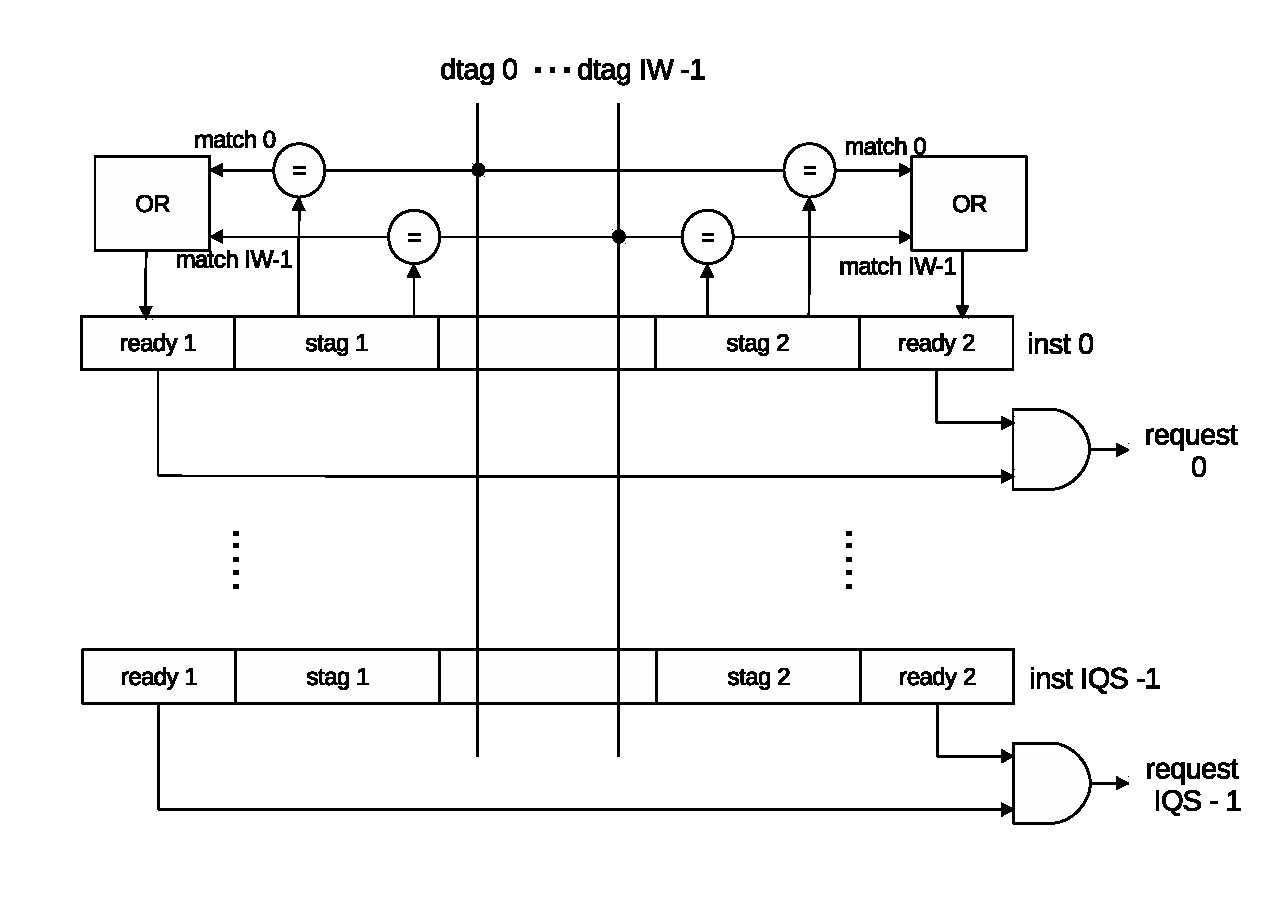
\includegraphics[keepaspectratio, scale=.8]{wakeup_logic}
  \caption{ウェイクアップ論理}
  \label{fig:wakeup_logic}
\end{figure}

\begin{figure}[htb]
  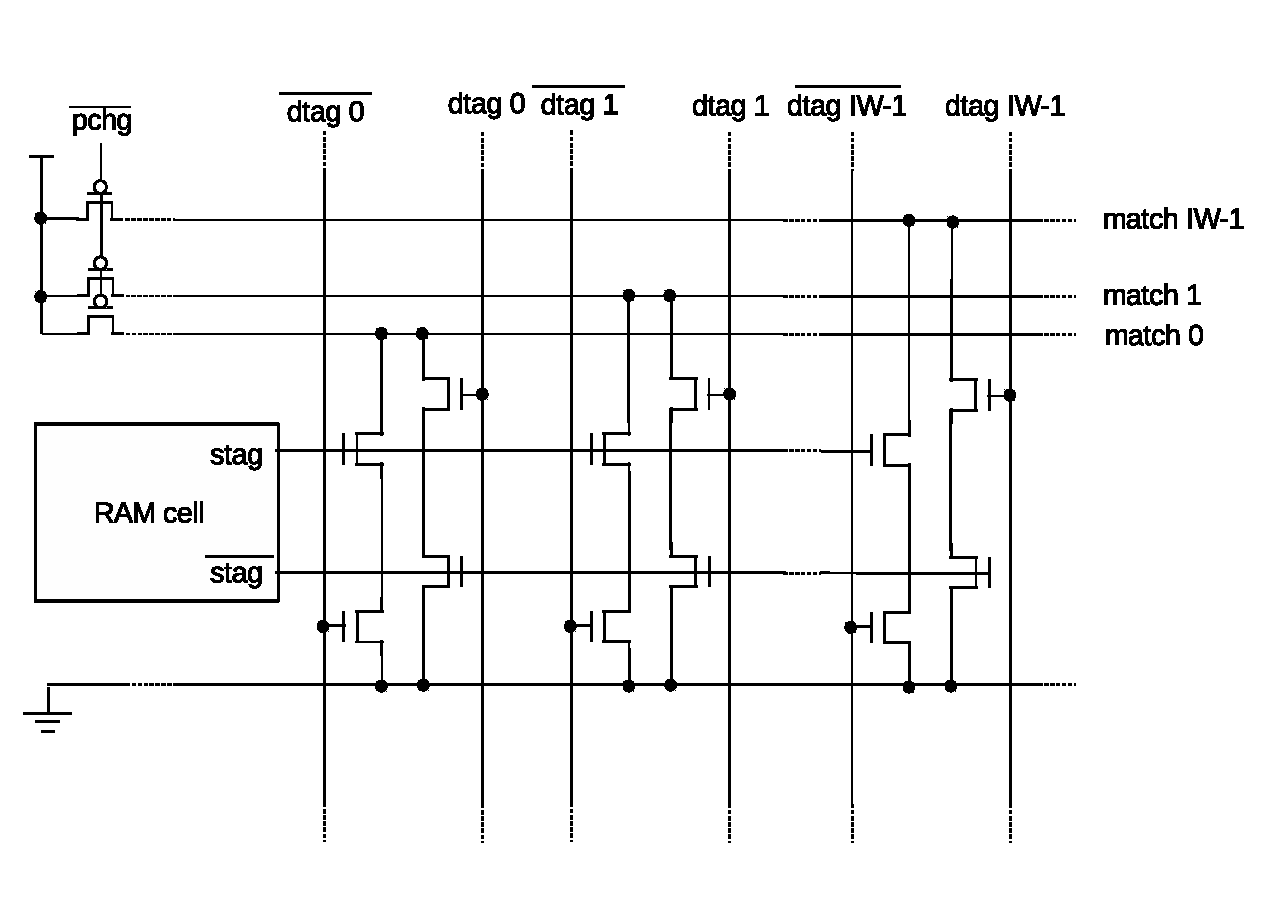
\includegraphics[keepaspectratio, scale=.8]{cam}
  \caption{タグ比較器の CAM 回路}
  \label{fig:cam}
\end{figure}

\subsection{ウェイクアップ論理}
\label{sec:wakeup_logic}
\fig{wakeup_logic}に,ウェイクアップの回路を示す.図中の $IW$ は発行幅を,$IQS$ は IQ のエントリ数を表す.ウェイクアップでは,$IW$ 個のディスティネーション・タグ(dtag)が IQ 内の全命令に放送される.各命令は 2 つのソース・タグ(stag)を保持しており,放送されたディスティネーション・タグと比較が行われる.いずれかのディスティネーション・タグとソース・タグが一致した場合,そのソース・オペランドのレディ・ビットがセットされる.2 つのレディ・ビットがセットされた命令は発行が可能となるため発行要求が出力される.

\fig{cam}に,IQ に使用されるタグ比較器の CAM 回路を示す.同図は,ソース・タグ 1 ビット分の比較回路を表す.同図に示すように,高速化のため通常ダイナミック論理によって構成される.比較の動作は,次のように行われる.まず,マッチ線がプリチャージされる.次にデスティネーション・タグが放送され,比較が行われる.タグが不一致であれば,直列に接続された 2 つのプルダウン・トランジスタが両方とも ON となり,マッチ線がディスチャージされる.タグが一致する場合,マッチ線は $H$ の状態が維持される.比較器はマッチ線のディスチャージ時に電力を消費する.

\section{IQ の方式}
\label{sec:iq_scheme}
これまで,IQ の方式としてシフト・キュー,サーキュラ・キュー,ランダム・キューの 3 つの方式が提案されている.各方式に関して説明したのち,現在主流な方式であるエイジ論理付きのランダム・キューに関して説明する.

\subsection{シフト・キュー}
シフト・キューは,最も古くに提案され,商用プロセッサに使用された IQ の方式である~\cite{Farrell1998}.シフト・キューでは,IQ の先頭のエントリより順に命令をディスパッチする.これにより,古い命令に高い発行優先度を与えることができる.\footnote{一般に,古い命令から優先的に発行すると,性能がより高くなることが知られている.}

また,シフト・キューでは命令を発行したエントリの空きを詰めるコンパクションを行うことにより,高い容量効率も達成することができる.正しい発行優先度と,高い容量効率を同時に達成するため,シフト・キューは IQ の方式の中で最も高い性能を得ることができる.

一方でシフト・キューには,コンパクションの回路が非常に複雑で,また消費電力が非常に大きいという欠点がある.そのため,シフト・キューはスケーリングが困難となっており,現在のプロセッサには使用されていない.

\subsection{サーキュラー・キュー}
サーキュラー・キューは,命令をプログラム順に並べるが,コンパクションを行わないような方式である~\cite{Abella:survey2003}.IQ は,ヘッド・ポインタとテール・ポインタを用いてサーキュラー・バッファとして管理される.

サーキュラー・キューでは,既に命令が発行されているが,新たに命令をディスパッチできないエントリが発生するため,IQ の容量効率がシフト・キューと比較して低下する.また,ヘッド・ポインタとテール・ポインタの位置が逆転するラップ・アラウンドが生じた際には,新しい命令に高い優先度が与えられる優先度逆転が起き,選択論理が正しい優先度で命令を選択できない.これらの理由から,サーキュラー・キューはシフト・キューと比較して性能が低下する.特に,容量効率が低下する影響は大きく,現在のプロセッサには使用されていない.

\subsection{ランダム・キュー}
近年は,回路の単純化や電力削減のため空いているエントリに単純にディスパッチするランダム・キューが使用されている~\cite{Alpha21464, AMD-Bulldozer, IBM-Power8}.ランダム・キューでは IQ の容量を無駄にすることがなく,高い容量効率を達成する.その一方で,命令が年齢とは無関係にランダムに並ぶため,正しい優先度で命令を発行することが出来ない.

ランダム・キューでは,IQ の空きエントリのインデクスを保持するフリー・リストを用意する.ディスパッチ時には,フリー・リストから読み出したインデクスが指す IQ のエントリに命令を書き込む.IQ から命令が発行されエントリが無効化されると,そのインデクスをフリー・リストへ返す.フリー・リストは FIFO バッファで管理される.

\subsection{エイジ論理付きランダム・キュー}
ランダム・キューにおける発行優先度の欠点を緩和するため,ランダム.キューは一般にエイジ論理と併用される~\cite{Alpha21464}.エイジ論理は選択論理と並列に動作する回路で,発行要求が出された命令の中で最も古い 1 命令を選ぶ.最も古い命令はクリティカル・パス上の命令である可能性が高いため,これを優先して発行することができ,結果としてエイジ論理付きランダム・キューは通常のランダム・キューと比較して性能が大きく向上する.

本研究における IQ は,エイジ論理付きのランダム・キューを使用する.



\chapter{関連研究}
\label{sec:related_work}
本章では,発行キュー(IQ:Issue Queue)に関連する研究について述べる.\refsec{relate_IQ}で IQ に関する一般的な関連研究に関して説明し,\refsec{relate_energy} で IQ の研究のうち,電力に関係する研究を述べる.

\section{IQ に関する関連研究}
\label{sec:relate_IQ}
Palacharla らは,命令発行幅と IQ のサイズを変化させた時の,ウェイクアップ論理と選択論理の遅延を評価した~\cite{Palacharla1997}.また,遅延を小さくするために,IQ を複数のFIFOバッファで構成し,依存する命令を同じFIFOバッファに割り当てる依存ベースの IQ を提案した.この手法では,各バッファの先頭の命令のみ発行可能かチェックすれば良いので,回路が単純化され遅延が減少する.

Stark らは,IPC をほとんど低下させずに,ウェイクアップ論理と選択論理をパイプライン化する手法を提案した~\cite{Stark2000}.この手法では,投機的にウェイクアップを行うことで,依存する命令を連続するサイクルで発行できるようにした.

五島らは,ウェイクアップ論理を従来の CAM ではなく,依存行列と呼ぶ RAM で構成する手法を提案した~\cite{goshima2001}.これによって比較器を用いずに依存する命令をウェイクアップすることが可能で,ウェイクアップの遅延を短縮できる.

Sassone らは,依存行列の遅延と電力をより小さくするための手法を提案した~\cite{sassone2007}.具体的には,従来はすべての命令について,その古さを完全に追跡していたのに対して,命令をグループ化してグループ単位で古いものを選択する.これにより,性能低下を最小限に抑えながら,回路の規模を小さくできる.

Lebeck らは.キャッシュ・ミスするロードのような長いレイテンシの命令に依存する命令を,IQ とは別の待機用バッファに入れ,その長いレイテンシの処理が完了するまで IQ に挿入しないという方式を提案した~\cite{Lebeck2002}.これによって,IQ が待機する命令で埋ることによって起こるストールの頻度が減り,性能が向上する.

Raasch らは,IQ をいくつかのセグメントに分割する方式を提案した~\cite{Raasch2002}.この方式では,各命令の依存命令チェーンのレイテンシを元に割り当てるセグメントが決定される.そして,発行可能になる直前に最下位セグメントである発行バッファに命令を移動する.この発行バッファでのみ発行を行うことで,すべてのエントリから発行できる通常の IQ と比較して遅延を短縮できる.

Kim らは,レイテンシが互いに1サイクルの依存関係のある2つの命令をグループ化し,1つの命令として IQ のエントリでスケジューリングすることで,依存グラフのエッジのレイテンシ短縮とキューの容量効率を上げる手法を提案した~\cite{Kim2003}.

Gibson らは,依存する命令をポインタでつなぎ,ポインタをたどることでウェイクアップを行う手法を提案した~\cite{Gibson2010}.この方式により CAM が不要になり,電力を削減できる.

安藤は,実行プログラムの命令レベル並列性(ILP:instruction-level parallelism)とメモリ・レベル並列性(MLP:memory-level parallelism)に応じて IQ の方式を切り替える手法を提案した~\cite{Ando2019}.ILP と MLP のいずれかが高い場合は IQ の容量効率が重要であるため,IQ をランダム・キューに構成する.ILP と MLP のどちらも低い場合には,容量効率よりも正しい発行優先度が重要であるため IQ をサーキュラー・キューに構成する.

甲良らは,実行プログラムの ILP と MLP に応じて IQ のサイズを変化させる手法を提案した~\cite{Kora2013}.本手法では,MLP が高い場合には,IQ の容量が重要となるため IQ のエントリ数を増加しパイプライン化する.MLP が低い場合には IQ のエントリ数を減少させ,パイプライン化を解除する.

\section{IQ の電力削減に関する関連研究}
\label{sec:relate_energy}
Folegnani らは,空のエントリの比較器や既にレディなオペランドを持つ比較器など,タグを比較する必要がない比較器を動作させないことで,消費エネルギーを削減する手法を提案した~\cite{folegnani2001}.

Ponomarev らは,リソース要求に応じて IQ のサイズをリサイズすることにより,消費エネルギーを削減する手法を提案した~\cite{ponomarev2001} .

Ernst らは,IQ に入ってくる命令のうちのほとんどが,はじめから少なくとも1つのソース・オペランドがレディであると指摘した~\cite{ernst2002}.そして IQ に,2つのソース・オペランドを保持できるエントリに加えて,1つのソース・オペランドのみ保持できるエントリと,ソース・オペランドを保持しないエントリを用意し,レディでないソース・オペランドの数に応じていずれかにディスパッチする手法を提案した.さらにこの手法を実現するために,命令の2つのオペランドの内,あとにレディになるオペランドを予測する手法も提案した.

Sembrant らは,クリティカル・パス上にない命令を IQ とは別のバッファに入れ,ディスパッチを遅延させることによって,性能を低下させずに IQ のサイズを小さくする手法を提案した~\cite{Sembrant2015}.

Homayoun らは,キャッシュ・ミスの処理中に発行幅を半減させることで,IQ の消費電力を削減する手法を提案した~\cite{H.Homayoun2011}.発行幅半減中に元の発行幅の半分以上の命令が発行される場合,一時的にその命令を小さなバッファに移動させることで対応している.

小林,松田らは,ウェイクアップ時のタグ比較を 2 段階に分割することによりエネルギー削減を行う方法を提案した~\cite{kobayashi-thesis, matsuda-thesis}.この方法では,タグの比較を高位ビットと低位ビットに分割し,低位ビットの比較を最初のサイクルで行う.そして低位ビットが一致していた場合のみ,次のサイクルで高位ビットの比較を行う.低位ビットの比較で一致しない場合,高位ビットの比較は行われず,エネルギーを削減することができる.また,タグの 2 段階比較には,ウェイクアップに 2 サイクル必要であるため性能が低下するという欠点が存在する.これに対しこの手法では,クリティカル・パス上にあると推測される命令のみ 1 サイクルで比較を行い性能低下を軽減する.



\chapter{提案手法:セグメント化した IQ}
\label{sec:segment_IQ}

\section{発行キューのセグメント化}
\label{sec:segmented_IQ}
本論文では,発行キューのタグ比較器の動作回数を削減するための手法として,発行キューをセグメント化する手法を提案する.本節では,まず提案手法の概要を説明した後,提案手法におけるウェイクアップとディスパッチに関して詳しく説明する.

\begin{figure}[htb]
  \centering
  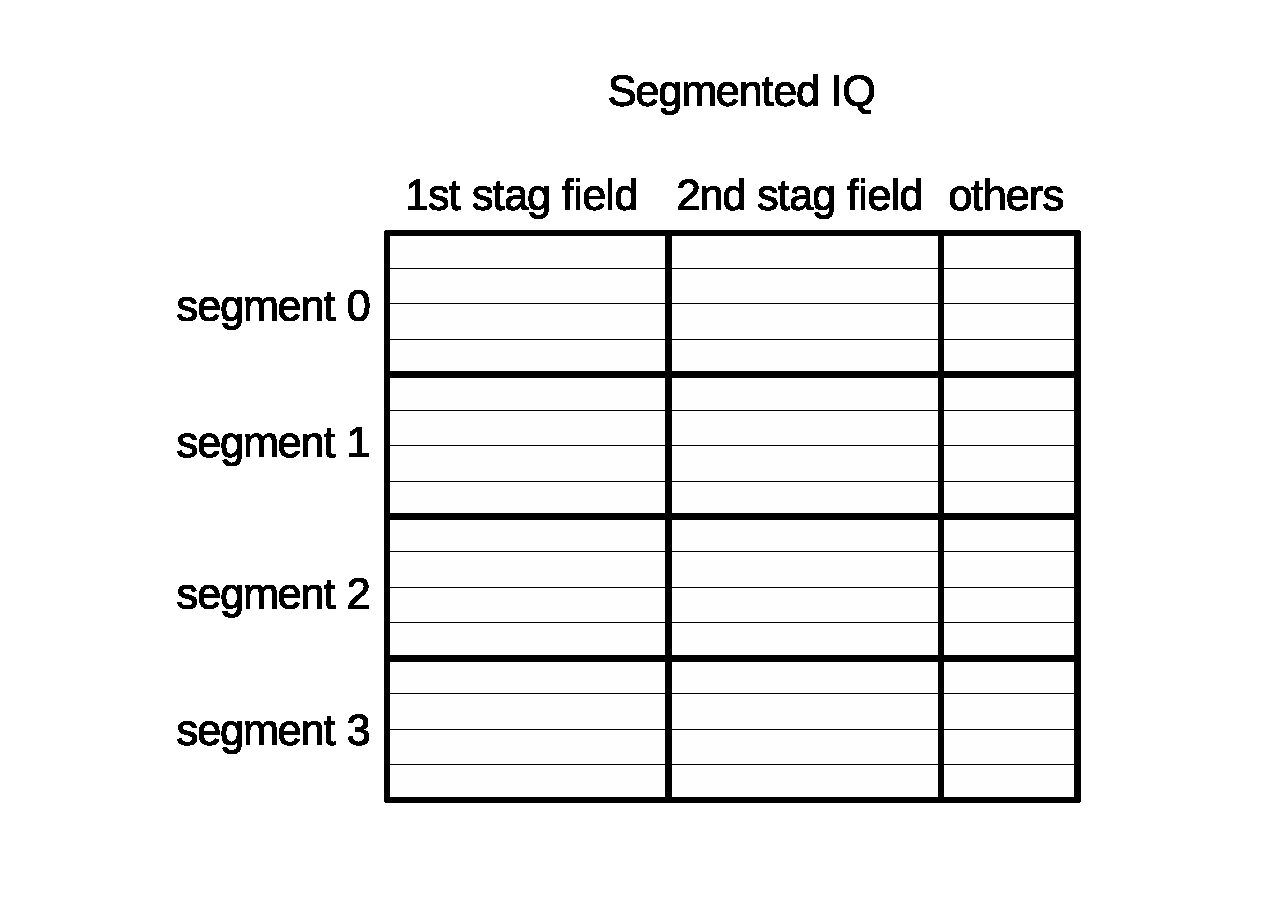
\includegraphics[keepaspectratio, scale=.8]{segmentedIQ}
  \caption{セグメント化した発行キュー}
  \label{fig:segmentedIQ}
\end{figure}

\subsection{提案手法の概要}
提案手法の基本アイデアは,大容量 CAM の電力削減に関する研究~\cite{Motomura1990paper,Motomura1990journal}から着想を得ている.この研究において提案されている手法では,CAM を複数の\textbf{セグメント}~\footnote{文献~\cite{Motomura1990paper,Motomura1990journal}ではバンクと呼ばれている}に分割する.各セグメントには下位ビットが同一のデータのみを記録する.そして,比較が行われる際には,比較対象のデータの下位ビットと,記録されているデータの下位ビットが一致するセグメントのみで比較を行う.これによって,比較器が動作する回数を「1/セグメント数」まで削減することができ,消費電力が削減できる.

本手法においても,\fig{segmentedIQ}に示すように発行キューを複数のセグメントに分割する.各セグメントには,第 1 ソース・タグの下位ビットがセグメントの番号と一致する命令をディスパッチする.ウェイクアップ時の第 1 ソース・タグのタグ比較では,ディスティネーション・タグの下位ビットとセグメントの番号が一致するセグメントのみでタグ比較を行う.これによって,第 1 ソース・タグのタグ比較回数を「1/セグメント数」に削減できる.

提案手法におけるディスパッチとウェイクアップに関して詳しく説明する.

\begin{figure}[tb]
  \centering
  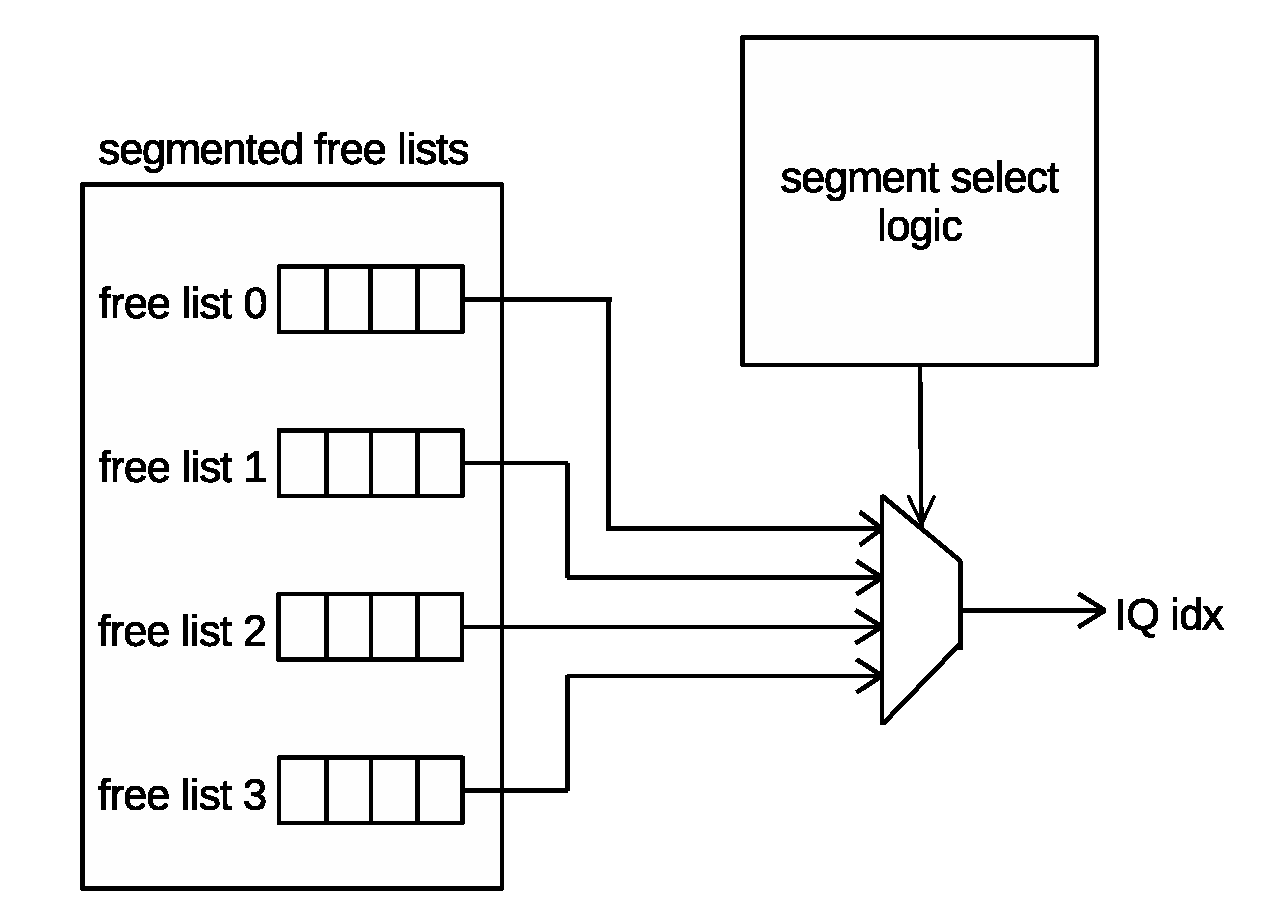
\includegraphics[keepaspectratio, scale=.8]{dispatch}
  \caption{提案手法におけるディスパッチエントリの決定回路}
  \label{fig:dispatch}
\end{figure}


\begin{figure*}[htb]
  \centering
  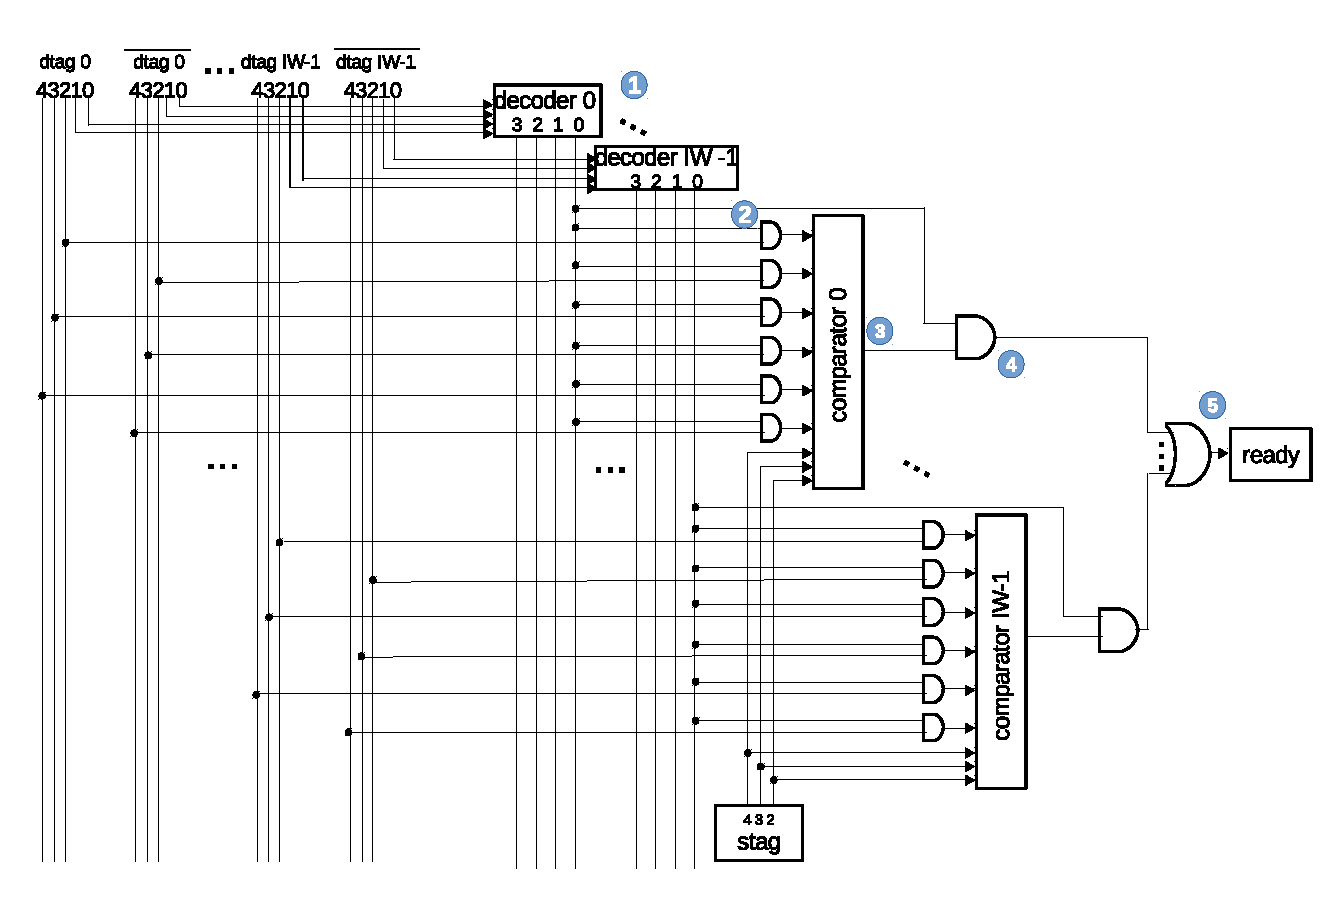
\includegraphics[width=0.80\hsize]{segmentedIQ_wakeup}
  \caption{提案手法におけるタグ比較回路(第 0 セグメント)}
  \label{fig:segmentedIQ_wakeup}
\end{figure*}

\subsection{提案手法におけるディスパッチ}
ディスパッチする発行キューのエントリを決定する回路を\fig{dispatch}に示す.本手法では,フリー・リストをセグメントと同じ数だけ用意する.各フリー・リストは,対応するセグメントの空きエントリのインデクスを FIFO バッファで管理する.各フリー・リストからは発行キューのインデクスが出力され,その中の1つを選択してディスパッチするエントリを決定する.どのフリー・リストからの出力を選択するかは,セグメント選択回路(図中の segment select logic)によって決定される.

セグメント選択回路の選択アルゴリズムについて説明する.セグメントの選択方法は,ディスパッチ時に第 1 ソース・オペランドがレディであるかによって異なるため,それぞれの場合に関して説明する.
\begin{itemize}
  \item \textbf{第 1 ソース・オペランドがレディでない場合}: 第 1 ソース・タグの下位ビットと番号が同じセグメントを選択する.選択されたセグメントに空きエントリがある場合,ディスパッチ可能であるため,対応するフリー・リストから読み出したエントリにディスパッチを行う.対応するセグメントに空きがない場合は,セグメントに空きが出るまでディスパッチをストールさせる.
  \item \textbf{第 1 ソース・オペランドがレディである場合}:この場合,第 1 ソース・タグの比較は行われないため,どのセグメントにディスパッチしても問題ない.このような場合を\textbf{セグメント・インディペンデント}と呼ぶ.セグメント・インディペンデントの場合,空きエントリのあるセグメントから,ラウンドロビンでディスパッチするセグメントを選択しディスパッチする.
\end{itemize}
例として,第 1 ソース・オペランドがレディでなく,タグが 15(${\rm 1111_2}$)である命令を,\fig{segmentedIQ}に示す 4 つに分割された発行キューにディスパッチする場合を考える.第 1 ソース・タグの下位 2 ビットが 3(${\rm 11_2}$)であるので,この命令は第 3 セグメントにディスパッチされる. 

なお,ソース・オペランドを使用しない命令も存在するが,そのような命令はディスパッチ時にソース・オペランドがレディであるものとして扱う.


\subsection{提案手法におけるウェイクアップ}
提案手法におけるウェイクアップでは,ディスティネーション・タグの下位ビットがセグメント番号と一致するセグメントでのみ,第 1 ソース・タグのタグ比較器を動作させ比較を行う.一致しないセグメントはタグ比較器を動作させない.これは,ディスティネーション・タグの下位ビットと番号が一致しないセグメントには,第 1 ソース・タグの下位ビットがディスティネーション・タグの下位ビットと異なる命令しか入っておらず,タグは必ず不一致となるためである.

例として,放送されたディスティネーション・タグが 6(${\rm 110_2}$)で,発行キューが\fig{segmentedIQ}のように 4 つのセグメントに分割されている場合を考える.この場合,下位ビットは 2(${\rm 10_2}$)であるため,第 2 セグメントでのみ,第 1 ソース・タグのタグ比較を行う.

なお,第 2 ソース・タグのタグ比較に関しては,セグメントの番号とタグの下位ビットに関係性はないため,すべてのセグメントでタグ比較を行う必要がある.

提案手法におけるタグ比較の回路を\fig{segmentedIQ_wakeup}に示す.同図は 4 つのセグメントに分割された発行キューのうち,第 0 セグメントのエントリにおける,第 1 ソース・タグの比較回路を示している.タグ・ビット数は 5 とし、発行幅を $IW$ とする.

タグ比較の動作を図中の番号を用いて説明する.\ctext{1}放送されるディスティネーション・タグの下位 2 ビットはデコーダへ送られる.デコーダはセグメント数だけ信号線を出力する.第 $n$ 番目の信号線は,第 $n$ セグメントでのタグ比較が有効であることを示す.つまり,ディスティネーション・タグの下位ビットが $n$ の場合,$n$ 番目の出力線のみ $H$ を出力し,残りはすべて $L$ を出力する.

\ctext{2}AND ゲートによって,デコーダからの信号線が $H$ の場合にのみ,ディスティネーション・タグの高位ビット及びその反転信号がタグ比較器へ入力される.\fig{segmentedIQ_wakeup}に示す回路は第 0 セグメントのタグ比較回路であるため,デコーダの 0 番目の信号線が AND ゲートに入力されている.

デコーダからの信号線が $H$ の場合,つまり,ディスティネーション・タグの下位ビットとセグメント番号が一致していた場合のみ,比較器に有効なディスティネーション・タグの高位ビットとその反転信号が送られ,ソース・タグの高位ビットと比較が行われる.デコーダからの信号線が $L$ の場合,ディスティネーション・タグとその反転信号がどちらも L としてタグ比較器へ入力される.この場合,ディスティネーション・タグとその反転信号に接続されたプルダウン・トランジスタがすべて OFF となるため,マッチ線はディスチャージされず,電力を消費しない.

\ctext{3}タグ比較の結果,タグの高位ビットが一致した場合は,比較器から $H$ が出力される.

\ctext{4}タグ比較器が $H$ を出力し,かつデコーダからの信号が $H$ である場合に,タグ比較は一致となる.

\ctext{5}いずれかのディスティネーション・タグがソース・タグと一致した場合に,ソース・オペランドのレディ・ビットがセットされる.


%4 第 2 ソース・タグ比較の削減
\section{第 2 ソース・タグ比較の削減}
\label{sec:second_tag_comp}
\ref{sec:segmented_IQ}節で述べた手法では,命令の第 2 ソース・タグのタグ比較回数は削減できない.そこで本節では,第 2 ソース・タグの比較回数の削減を可能とする\textbf{スワップ}と\textbf{サブ・セグメント}という 2 つの手法を提案する.

\subsection{スワップ}
\label{sec:swap}
スワップは,第 1 ソース・タグと第 2 ソース・タグを格納するフィールドを交換し,第 2 ソース・タグの下位ビットをもとにディスパッチするセグメントを決定する手法である.以下で詳しく説明する.

第 1 ソース・オペランドがレディで,第 2 ソース・オペランドがレディでない場合について説明する.この場合,\ref{sec:segmented_IQ}節で説明した方法では,命令はセグメント・インディペンデントとしてディスパッチされる.第 1 ソース・オペランドは既にレディであるため,比較は第 2 ソース・タグについてのみ行われるが,第 2  ソース・タグのタグ比較は全てのセグメントで行われるため,タグ比較の回数は削減されない.

そこでこのような場合に,第 1 ソース・タグと第 2 ソース・タグを交換し(スワップ),第 2 ソース・タグの下位ビットを使用してディスパッチするセグメントを選択する.これにより,\ref{sec:segmented_IQ}節で述べたセグメント化の効果でタグ比較回数が削減される.なお,スワップではタグを交換するが,ペイロード RAM に格納するソース・タグを交換するわけではないので,命令の意味は保持される.

\subsubsection{スワップを行う場合のセグメント選択アルゴリズム}
セグメント選択回路は,以下に示すアルゴリズムによってディスパッチするセグメントを決定する.
\begin{itemize}
  \item \textbf{両ソース・オペランドともレディでない場合}:第 1 ソース・タグでセグメントを選択する.
  \item \textbf{第 1 ソース・オペランドのみレディである場合}:スワップを行い,第 2 ソース・タグでセグメントを選択する.
  \item \textbf{第 2 ソース・オペランドのみレディである場合}:第 1 ソース・タグでセグメントを選択する.
  \item \textbf{両ソース・オペランドがレディである場合}:セグメント・インディペンデントとしてラウンドロビンでセグメントを選択する.
\end{itemize}
なお,両ソース・オペランドがレディのとき以外で,選択されたセグメントに空きがない場合は,ディスパッチをストールして当該のセグメントに空きが出るまで待ち合わせる.

\begin{figure}[htb]
  \centering
  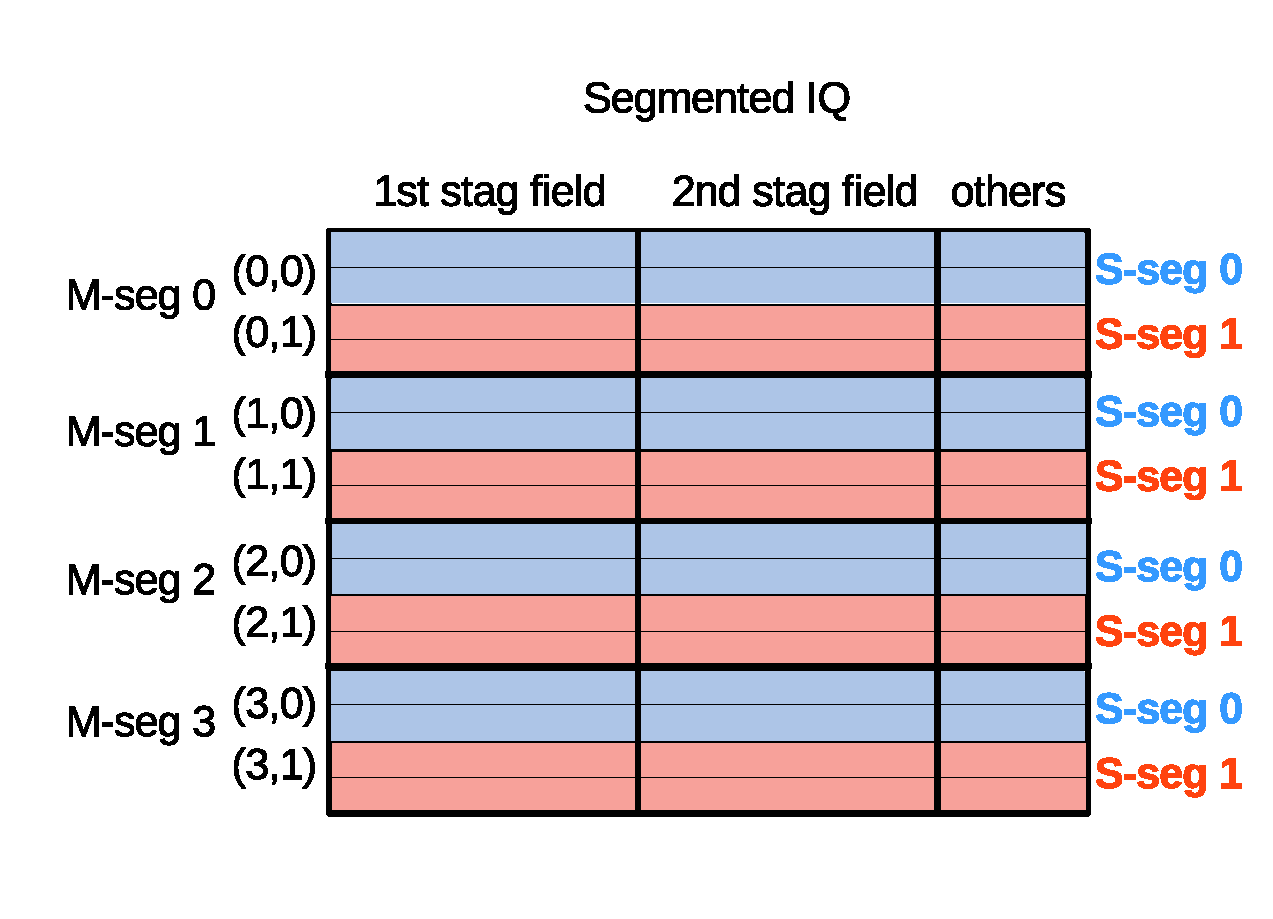
\includegraphics[keepaspectratio, scale=.8]{sub_segment}
  \caption{サブ・セグメントを実装した発行キュー}
  \label{fig:sub_segment}
\end{figure}

\subsection{サブ・セグメント}
\label{sec:sub_segment}
サブ・セグメント方式は,第 1 ソース・タグの下位ビットに応じて分割されるセグメントを,第 2 ソース・タグの下位ビットに応じてさらに細かく分割する.第 2 ソース・タグの下位ビットによる分割をサブ・セグメント(S-seg)と呼び,従来の第 1 ソース・タグによる分割をサブ・セグメントに対応してメイン・セグメント(M-seg)と呼ぶこととする.

サブ・セグメントを導入した発行キューの分割を\fig{sub_segment}に示す.黒色の枠で示す各メイン・セグメントを,赤色と青色で示すようにさらにサブ・セグメントに分割する.同図は,メイン・セグメント数が 4 ,サブ・セグメント数が 2 の場合の例を表している.各セグメントの左には,(M-seg, S-seg)という形式でメイン及びサブ・セグメントの番号を表している.

サブ・セグメント方式について,ディスパッチとウェイクアップの動作をそれぞれ説明する.

\subsubsection{サブ・セグメントにおけるディスパッチ}
サブ・セグメント方式におけるディスパッチにおいては,フリー・リストを M-seg $\times$ S-seg だけ用意する.\fig{sub_segment}に示した例の場合 8 個のフリー・リストが必要となる.

サブ・セグメント方式におけるセグメント選択のアルゴリズムに関して説明する.アルゴリズムはソース・オペランドのレディ状況によって異なるため,以下ですべての場合に関して説明する.説明を簡単にするため,命令 $p5 = p13 + p6$ を,\fig{sub_segment}に示す発行キューにディスパッチする場合について例示する.第 1 ソース・タグが 13 で,第 2 ソース・タグが 6 である.
\begin{itemize}
  \item \textbf{両ソース・オペランドともレディでない場合}:第 1 ソース・タグでメイン・セグメントを,第 2 ソース・タグでサブ・セグメントを選択する.例の場合,第 1 ソース・タグ 13(${\rm 1101_2}$) の下位ビット 1(${\rm 01_2}$)より,メイン・セグメントは 1 となる.また,第 2 ソース・タグ 6(${\rm 110_2}$) の下位ビット 0(${\rm 0_2}$)より,サブ・セグメントは 0 となる.従って(1, 0)のセグメントを選択する. 
  \item \textbf{第 1 ソース・オペランドのみレディである場合}:第 2 ソース・タグでサブ・セグメントを選択する.例の場合,第 2 ソース・タグ 6(${\rm 110_2}$) の下位ビット 0(${\rm 0_2}$)より,サブ・セグメントは 0 となる.第 1 ソース・オペランドは既にレディであるため,メイン・セグメントの制限はない.従って,(0, 0),(1, 0),(2, 0),(3, 0)のいずれかのセグメントをラウンドロビンで選択する.このように,メイン・セグメントの制限がない場合をメイン・セグメント・インディペンデント(M-seg インディペンデント)と呼ぶこととする.
  \item \textbf{第 2 ソース・オペランドのみレディである場合}:第 1 ソース・タグでメイン・セグメントを選択する.例の場合,第 1 ソース・タグ 13(${\rm 1101_2}$) の下位ビット 1(${\rm 01_2}$)より,メイン・セグメントは 1 となる.第 2 ソース・オペランドは既にレディであるため,サブ・セグメントの制限はない.従って,(1, 0)または(1, 1)のいずれかのセグメントをラウンドロビンで選択する.このように,サブ・セグメントの制限がない場合をサブ・セグメント・インディペンデント(S-seg インディペンデント)と呼ぶこととする.
  \item \textbf{両ソース・オペランドがレディである場合}:セグメント・インディペンデントとしてラウンドロビンでセグメントを選択する.
\end{itemize}

\subsubsection{サブ・セグメントにおけるウェイクアップ}
第 1 ソース・タグの比較は,ディスティネーション・タグの下位ビットがメイン・セグメント番号と一致するセグメントのみで行う.また,第 2 ソース・タグの比較は,ディスティネーション・タグの下位ビットがサブ・セグメント番号と一致するセグメントのみで行う.このような比較により,第 1 ソース・タグだけでなく,第 2  ソース・タグの比較に関しても,「1/サブ・セグメント数」まで削減が可能となる.

\subsubsection{サブ・セグメントとスワップの併用}
サブ・セグメント方式はスワップと併用することが可能である.併用する場合は,ディスパッチ時に第 1 ソース・オペランドのみレディである場合の選択アルゴリズムを,以下のように変更する.
\begin{itemize}
  \item \textbf{第 1 ソース・オペランドのみレディである場合}:スワップを行い,第 2 ソース・タグでメイン・セグメントを選択する.例の場合,第 2 ソース・タグ 6(${\rm 110_2}$) の下位ビット 2(${\rm 10_2}$)より,メイン・セグメントは 2 となる.第 1 ソース・オペランドは既にレディであるため,S-seg インディペンデントである.従って,(2, 0)または(2, 1)のいずれかのセグメントを選択する.
\end{itemize}
サブ・セグメント方式とスワップを併用することによって,ディスパッチ時に第 1 ソース・オペランドのみレディである命令におけるタグ比較回数の削減が「1/サブ・セグメント数」から「1/メイン・セグメント数」となる.従って,\fig{sub_segment}に示した分割のようにメイン・セグメント数がサブ・セグメント数よりも多い場合に,タグ比較回数をより多く削減できる.










% 図を使う例: figure 環境を使用

% \begin{figure}[tb]
%   \centering
%   \includegraphics[scale=.5]{hoge.eps}
%   \caption{例1}
%   \label{fig:hoge}
% \end{figure}



% 副図を使う例: minipage と subcaption を使用

% \begin{figure}[tb]
%   \begin{minipage}[htb]{1\hsize}
%     \centering 
%     \includegraphics[keepaspectratio, scale=0.8]{hap_pipeline.eps}
%     \vspace{.3cm} % <-- vspace で縦方向の位置を調節できる
%     \subcaption{従来のパイプライン (HAP: Hit-Assuming Pipeline)}
%     \label{fig:hap_pipeline}
%   \end{minipage}
%   \begin{minipage}[htb]{.97\hsize}
%     \vspace{1.3cm}
%     \centering
%     \includegraphics[keepaspectratio, scale=0.8]{map_pipeline.eps}
%     \vspace{.3cm}
%     \subcaption{MAP: Miss-Assuming Pipeline}
%     \label{fig:map_pipeline}
%   \end{minipage}
%   \vspace{.8cm}
%   \caption{各パイプラインの命令処理工程}
%   \label{fig:pipeline}
% \end{figure}



\chapter{SWITCH 方式}
\label{sec:switch}

\begin{figure}[tb]
  \centering
  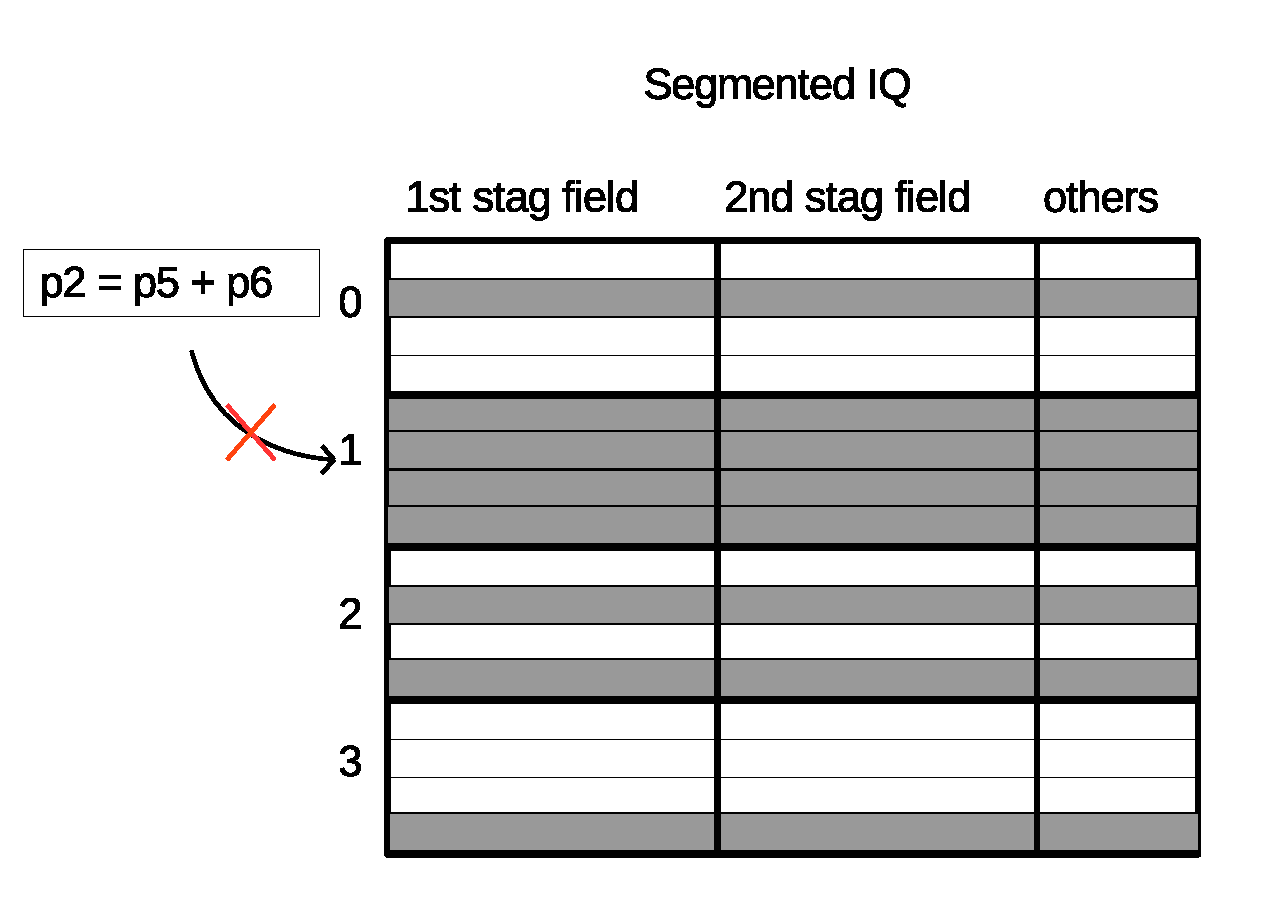
\includegraphics[keepaspectratio, scale=.8]{stall_segmentedIQ}
  \caption{容量効率が低下する例}
  \label{fig:stall_segmentedIQ}
\end{figure}


\section{容量効率の低下}
\label{sec:occupency_reduction}
提案手法には発行キューの容量効率が低下するという問題点がある.この問題点は,発行キューの容量効率が重要なプログラムにおいて,性能低下を引き起こす.本節では,容量効率が低下する原因について説明した後,容量効率の低下により性能低下を引き起こすプログラムの特徴に関して説明する.

\subsection{提案手法による容量効率低下の原因}
発行キューの容量効率の低下に関して,\fig{stall_segmentedIQ}を用いて説明する.図において,灰色のエントリは命令を保持していることを示している.

図の状態の発行キューに,新たに命令 $p2 = p5 + p6$ をディスパッチする場合を考える.この命令のソース・オペランドは両方レディでないとする.この場合,第 1 ソース・タグの下位ビットから第 1 セグメントにディスパッチされることが決定する.しかし,第 1 セグメントに空きエントリはないため,空きが出るまでディスパッチをストールさせ,待ち合わせを行う必要がある.

このように,命令がディスパッチされるセグメントに空きがない場合,他のセグメントに空きがあってもディスパッチをストールする必要があり,その結果,提案手法ではセグメント化されていない発行キューと比較して容量効率が低下する.

\subsection{容量効率の低下による性能低下}
プログラムには,性能が発行キューの容量に敏感なものとそうでないものとがある~\cite{Ando2019, Kora2013, Sembrant2015}.次の 2 つの特徴のうちいずれかに当てはまるプログラムでは,性能が発行キューの容量に敏感なため,与えられた発行キューの容量においては,その利用効率が重要である.このため,提案手法による容量効率の低下によって性能が低下する.
\begin{itemize}
  \item \textbf{命令レベル並列性(ILP:Instruction Level Parallelism)}が高いプログラム
  \item \textbf{メモリ・レベル並列性(MLP:Memory Level Parallelism)}が高いプログラム 
\end{itemize}

ILP が高いプログラムでは,できるだけ発行キューに命令を多く供給し,より多くの命令を並列に発行できるようにすることで高い性能が得られる.発行キューの容量効率が低下すると,並列に発行できる命令数が減少するため,性能が低下する.

MLP が高いプログラムでは,できるだけ多くのキャッシュ・ミスを並列に実行することにより,メモリ・アクセスのレイテンシが実行時間に与える影響を縮小できる.発行キューの容量効率が低下すると,並列に処理できるメモリ・アクセスが減少するため,性能が低下する.

これらのことから,ILP もしくは MLP が高い場合には,提案手法による容量効率の低下を最小限に抑える工夫が必要となる.

%5 容量効率の低下への対策:SWITCH 方式
\section{容量効率低下への対策:SWITCH 方式}
\label{sec:switch}
発行キューの容量効率低下による性能低下を抑制する方式として,\textbf{SWITCH} と呼ぶ方式を提案する.SWITCH 方式では,次のようにして性能低下を抑制する.
\begin{itemize}
  \item セグメント選択回路の選択アルゴリズムとして,容量効率は低下するが,タグ比較回数を多く削減できるような選択を行う \textbf{AGGRESSIVE モード} と,タグ比較回数の削減率は低下するが,容量効率が大きく低下しないような選択を行う \textbf{CONSERVATIVE モード} の 2 つを用意する.
  \item 実行プログラムの ILP 及び MLP を一定のインターバルで監視し,ILP もしくは MLP が高いと判断されたなら次のインターバルでは CONSERVATIVE モードでディスパッチし,そうでないなら AGGRESSIVE モードでディスパッチを行う.
\end{itemize}

本節では,まず 2 つのセグメント選択のアルゴリズムに関して説明を行う.その後,ILP 及び MLP の評価方法と,切り替えアルゴリズムに関して説明する.

\subsection{2 つのセグメント選択アルゴリズム}
\label{sec:two_mode}
SWITCH 方式では,タグ比較回数の削減重視の AGGRESSIVE モードと,容量効率重視の CONSERVATIVE モードの 2 つを適切に切り替えて使用する.各モードには,タグ比較回数の削減と容量効率に関して,\tab{switch_trade_off}に示すトレード・オフの関係がある.それぞれのセグメントの選択方法に関して説明する.

なお, SWITCH 方式はサブ・セグメントと併用が可能である.まず,サブ・セグメントを使用しない場合の AGGRESSIVE 及び CONSERVATIVE のアルゴリズムに関した説明したのち,サブ・セグメントと併用する場合のアルゴリズムへと拡張して説明する.

\begin{table}[tb]
  \caption{2 つのセグメント選択モードのトレード・オフ}
  \footnotesize
  \center
   \begin{tabular}{l|c|c} \hline \hline
   モード & タグ比較回数の削減 & 容量効率 \\ \hline
   AGGRESSIVE & ○ & × \\
   CONSERVATIVE & × & ○ \\ \hline
  \end{tabular}
  \label{tab:switch_trade_off}
\end{table}

\subsubsection{AGGRESSIVE モード}
AGGRESSIVE モードは,\tab{agg_algorithm}で示した選択アルゴリズムを使用してディスパッチするエントリを決定する.このモードでは,選択されたセグメントに空きがない場合,他のセグメントに空きがあってもディスパッチは行わないため,容量効率が低下する.しかし,セグメント化の利益を最大限利用し,タグ比較回数を大幅に削減できる.

\subsubsection{CONSERVATIVE モード}
AGGRESSIVE モードでは,命令のソース・オペランドが両方レディであり,セグメント・インディペンデントとしてディスパッチできる場合以外では,ソース・タグによって選択されるセグメントに空きがない場合にディスパッチをストールさせる.これに対し,CONSERVATIVE モードでは,以下で説明する工夫を行うことによって,このディスパッチのストールを回避し,容量効率の低下を抑制する.
\begin{itemize}
  \item \textbf{両ソース・オペランドともレディでない場合}:\\AGGRESSIVE モードでは第 1 ソース・タグの下位ビットによってセグメントを選択する.選択されたセグメントに空きがない場合,ディスパッチを行わない.これに対して CONSERVATIVE モードでは,第 1 ソース・タグによって選択されたセグメントに空きがない場合には,\textbf{スワップ}~\footnote{\ref{sec:swap}節では,スワップの定義を「第 1 ソース・オペランドのみレディの場合に,第 1 ソース・タグと第 2 ソース・タグを書き込むフィールドを交換する」としていたが,本節以降ではこの定義を拡大し,単に「第 1 ソース・タグと第 2 ソース・タグを書き込むフィールドを交換する」という意味で用いる.}\textbf{して}ディスパッチを試みる.スワップするため,第 2 ソース・タグにより選択されるセグメントに空きがあればディスパッチが可能となる.
  \item \textbf{第 1 ソース・オペランドのみレディである場合}:\\AGGRESSIVE モードでは,スワップを行い,第 2 ソース・タグでセグメントを選択する.選択されたセグメントに空きがない場合,ディスパッチを行わない.これに対して CONSERVATIVE モードでは,第 2 ソース・タグによって選択されたセグメントに空きがない場合には,\textbf{スワップをやめて}ディスパッチする.スワップをやめるため,第 1 ソース・タグによってセグメントが選択されるが,第 1 ソース・オペランドは既にレディであるため,どのセグメントにディスパッチしても良い.従って,セグメント・インディペンデントとしてディスパッチが可能となる.
  \item \textbf{第 2 ソース・オペランドのみレディである場合}:\\AGGRESSIVE モードでは第 1 ソース・タグでセグメントを選択する.選択されたセグメントに空きがない場合,ディスパッチを行わない.これに対して CONSERVATIVE モードでは,第 1 ソース・タグによって選択されたセグメントに空きがない場合には,\textbf{スワップして}ディスパッチする.スワップするため,第 2 ソース・タグによってセグメントが選択されるが,第 2 ソース・オペランドは既にレディであるため,どのセグメントにディスパッチしても良い.従って,セグメント・インディペンデントとしてディスパッチが可能となる.
\end{itemize}
上述の工夫によって,CONSERVATIVE モードでは,どちらかのソース・オペランドがレディである場合は,必ずディスパッチが可能となる.また,両ソース・オペランドともレディでない場合でも,第 1 ソース・タグにより選択されるセグメントと第 2 ソース・タグにより選択されるセグメントのうち,いずれかのセグメントに空きがあればディスパッチが可能となる.従って,ストールする確率は大きく減少する.

\tab{cons_algorithm}に,CONSERVATIVE モードにおけるセグメントの選択アルゴリズムをまとめる.

\begin{table}[htb]
  \caption{CONSERVATIVE モードのセグメント選択アルゴリズム}
  \footnotesize
  \center
   \begin{tabular}{|c|p{13.5cm}|} \hline \hline
    ソース・タグの状態 & アルゴリズム \\ \hline
    (NR,NR) & 第 1 ソース・タグでセグメントを選択.選択したセグメントに空きがない場合, スワップして第 2 ソース・タグをもとにセグメントを決定.なおも空きがない場合はストール. \\ \hline
    (R,NR) & スワップを行い,第 2 ソース・タグでセグメントを選択.選択したセグメントに空きがない場合,スワップをやめてセグメント・インディペンデントとしてセグメントを選択する.\\ \hline
    (NR,R) & 第 1 ソース・タグでセグメントを選択.選択したセグメントに空きがない場合,スワップを行いセグメント・インディペンデントとしてセグメントを選択.\\ \hline
    (R,R) & セグメント・インディペンデントとしてセグメントを選択. \\ \hline
  \end{tabular}
  \label{tab:cons_algorithm}
\end{table}

% \begin{itemize}
%   \item \textbf{両ソース・オペランドともレディでない場合}:第 1 ソース・タグでセグメントを選択する.選択したセグメントに空きがない場合,スワップして第 2 ソース・タグをもとにセグメントを決定する.なおも空きがない場合はストールする.
%   \item \textbf{第 1 ソース・オペランドのみレディである場合}:スワップを行い,第 2 ソース・タグでセグメントを選択する.選択したセグメントに空きがない場合は,スワップをやめて,セグメント・インディペンデントとしてラウンドロビンでセグメントを選択する.
%   \item \textbf{第 2 ソース・オペランドのみレディである場合}:第 1 ソース・タグでセグメントを選択する.選択したセグメントに空きがない場合はスワップを行い,セグメント・インディペンデントとしてラウンドロビンでセグメントを選択する.
%   \item \textbf{両ソース・オペランドがレディである場合}:セグメント・インディペンデントとしてラウンドロビンでセグメントを選択する.
% \end{itemize}

\subsubsection{CONSERVATIVE モードにおけるタグ比較回数の削減}
CONSERVATIVE モードでは,AGGRESSIVE モードと比較してタグ比較回数の削減率が 低下する可能性がある.この理由について説明する.例として,第 2 ソース・オペランドのみレディである命令をディスパッチする場合について説明する.

CONSERVATIVE モードでは,まず第 1 ソース・タグでセグメントを選択する.選択されたセグメントに空きがあれば,そのセグメントにディスパッチする.この場合,レディでない第 1 ソース・タグが,セグメント化によってタグ比較回数が削減される第 1 ソース・タグのフィールドに書き込まれるため,AGGRESSIVE モードと同様にタグ比較回数が削減される.

第 1 ソース・タグによって選択されたセグメントに空きがなければ,CONSERVATIVE モードではスワップしてセグメント・インディペンデントとしてディスパッチする.この場合,タグ比較回数の削減は行うことができない.これは,既にレディである第 2 ソース・オペランドのタグが,セグメント化によってタグ比較回数を削減できる第 1 ソース・タグのフィールドに書き込まれ,一方で,まだレディでなくタグ比較が行われる第 2 ソース・オペランドのタグが,セグメント化によってタグ比較回数が削減されない第 2 ソース・タグのフィールドに書き込まれるためである.

AGGRESSIVE モードでは,第 1 ソース・タグによって選択されたセグメントに空きがなければ,ストールして空きが出るまで待ち合わせる.このストールにより,容量効率は低下するが,空きが出たあとディスパッチするため,タグ比較回数は削減される.これに対して CONSERVATIVE モードでは,タグ比較回数の削減は行えなくなるが,スワップしてディスパッチすることによってストールを回避し,容量効率の低下を防ぐ.

従って,CONSERVATIVE モードは,タグ比較回数の削減をある程度犠牲にして,発行キューの容量効率の低下を抑制するアルゴリズムであるといえる.

\subsubsection{サブ・セグメントとの併用}
SWITCH 方式とサブ・セグメントを併用する際の,2 つのモードのディスパッチ・アルゴリズムの拡張に関して説明する.

AGGRESSIVE モードに関しては,\tab{agg_algorithm_subseg}で示したアルゴリズムがそのまま サブ・セグメントを併用する場合の AGGRESSIVE モードでのアルゴリズムとなる.

CONSERVATIVE モードのアルゴリズムを,\tab{cons_algorithm_subseg}に示す.
\begin{table}[htb]
  \caption{CONSERVATIVE モードのセグメント選択アルゴリズム(サブ・セグメントと併用)}
  \footnotesize
  \center
   \begin{tabular}{|c|p{13.5cm}|} \hline \hline
    ソース・タグの状態 & アルゴリズム \\ \hline
    (NR,NR) & 第 1 ソース・タグでメイン・セグメントを,第 2 ソース・タグでサブ・セグメントを選択.選択したセグメントに空きがない場合, スワップして第 2 ソース・タグでメイン・セグメントを,第 1 ソース・タグでサブ・セグメントを決定.なおも空きがない場合はストール. \\ \hline
    (R,NR) & スワップを行い,第 2 ソース・タグでメイン・セグメントを選択し,S-seg インディペンデントとしてセグメントを選択.選択したセグメントに空きがない場合,スワップをやめ,第 2 ソース・タグでサブ・セグメントを選択し,M-seg インディペンデントとしてセグメントを選択.\\ \hline
    (NR,R) & 第 1 ソース・タグでメイン・セグメントを選択し,S-seg インディペンデントとしてセグメントを選択.選択したセグメントに空きがない場合,スワップして,第 1 ソース・タグでサブ・セグメントを選択し,M-seg インディペンデントとしてセグメントを選択.\\ \hline
    (R,R) & セグメント・インディペンデントとしてセグメントを選択. \\ \hline
  \end{tabular}
  \label{tab:cons_algorithm_subseg}
\end{table}
サブ・セグメントを使用するCONSERVATIVE モードのアルゴリズムは複雑であるが,基本的なアイデアはサブセグメントを使用しない場合と同じである.すなわち,選択されたセグメントに空きがない場合には,スワップを行い(あるいはスワップをやめて),再度セグメントの選択を行う.

(NR, NR),(R, NR),(NR, R)に関して,例を用いて以下で説明する.メイン・セグメント数を 4,サブ・セグメント数を 2 とし,命令 $p5 = p13 + p6$ をディスパッチする場合について例示する.第 1 ソース・タグが 13 で,第 2 ソース・タグが 6 である.
\begin{itemize}
  \item \textbf{(NR,NR)}:第 1 ソース・タグでメイン・セグメントを,第 2 ソース・タグでサブ・セグメントを選択する.この場合,第 1 ソース・タグ 13(${\rm 1101_2}$),第 2 ソース・タグ 6(${\rm 110_2}$)より,(1, 0)のセグメントを選択する. もし(1,0)に空きがない場合はスワップを行い,第 2 ソース・タグでメイン・セグメントを,第 1 ソース・タグでサブ・セグメントを選択する.この場合,(2, 1)が選択される.なおも空きがない場合はストールする.
  \item \textbf{(R,NR)}:スワップを行い,第 2 ソース・タグでメイン・セグメントを選択する.例の場合,第 2 ソース・タグ 6(${\rm 110_2}$)より,メイン・セグメントは 2 となる.第 1 ソース・オペランドは既にレディであるため,S-seg インディペンデントである.従って,(2, 0)または(2, 1)のいずれかのセグメントを選択する.(2, 0)と(2,1)のいずれも空きがない場合は,スワップをやめ,第 2 ソース・タグでサブ・セグメントを決定する.この場合,サブ・セグメントは 0 となる.第 1 ソース・オペランドは既にレディであるため,M-seg インディペンデントである.したがって(0,0),(1,0),(2,0),(3,0)のいずれかのセグメントが選択される.なおも空きがない場合はストールする.
  \item \textbf{(NR,R)}:第 1 ソース・タグでメイン・セグメントを選択する.例の場合,第 1 ソース・タグ 13(${\rm 1101_2}$)より,メイン・セグメントは 1 となる.第 2 ソース・オペランドは既にレディであるため,S-seg インディペンデントである.従って,(1, 0)または(1, 1)のいずれかのセグメントを選択する.(1, 0)と(1, 1)のいずれも空きがない場合は,スワップを行い,第 1 ソース・タグでサブ・セグメントを決定する.この場合,サブ・セグメントは 1 となる.第 2 ソース・オペランドは既にレディであるため,M-seg インディペンデントである.したがって(0,1),(1,1),(2,1),(3,1)のいずれかのセグメントが選択される.なおも空きがない場合はストールする.
\end{itemize}


\subsection{モードの切り替え}
SWITCH 方式では, AGGRESSIVE と CONSERVATIVE の 2 つのモードを,実行プログラムの ILP や MLP の量に応じて切り替えて使用する.ここで重要となるのは ILP や MLP の量の評価方法である.

本研究では, ILP の評価方法としてIPC(Instructions Per Cycle)と Issue Stall Rate(ISR) という評価値が有効でないかと考えた.また, MLP の評価方法としては,最終レベル・キャッシュ(LLC: last-level cache)の MPKI(misses per kilo instructions)が有効ではないかと考えた.それぞれに関して詳しく説明した後,切り替えアルゴリズムを説明する.

なお,評価の結果 ILP を評価する評価値としては ISR がより適しているとわかったため,ISR を ILP の評価値として使用する.これらの評価は\refsec{eval_switch}で説明する.

\subsubsection{Instructions Per Cycle(IPC)}
IPC は,サイクルあたりの平均コミット命令数を表す指標であり,プロセッサの性能指標として一般的に使用される評価値である.IPC が高い場合,ILP は高いと判断される.

あらかじめ IPC にしきい値を設け,インターバルでの IPC がしきい値を上回った場合に ILP が高いと判断し,そうでなければ低いと判断する.

\subsubsection{Issue Stall Rate(ISR)}
ISR は,「インターバルの全サイクルのうち 1 命令も発行されないサイクルの割合」を表す指標である.ILP が高い場合,多くのサイクルで命令が発行されるため,ISR は低い値を示す.一方, ILP が低い場合には,命令が発行されないサイクルが一定の割合で発生するため,ISR は高くなる.

あらかじめISR にしきい値を設け,インターバルでの ISR がしきい値を下回った場合に ILP が高いと判断し,そうでなければ低いと判断する.

\subsubsection{LLC MPKI}
LLC MPKI は LLC のキャッシュ・ミスの発生頻度を表す指標である.LLC MPKI があらかじめ定めたしきい値を上回った場合に MLP が高いと判断し,そうでなければ低いと判断する.

\begin{figure}[htb]
  \centering
  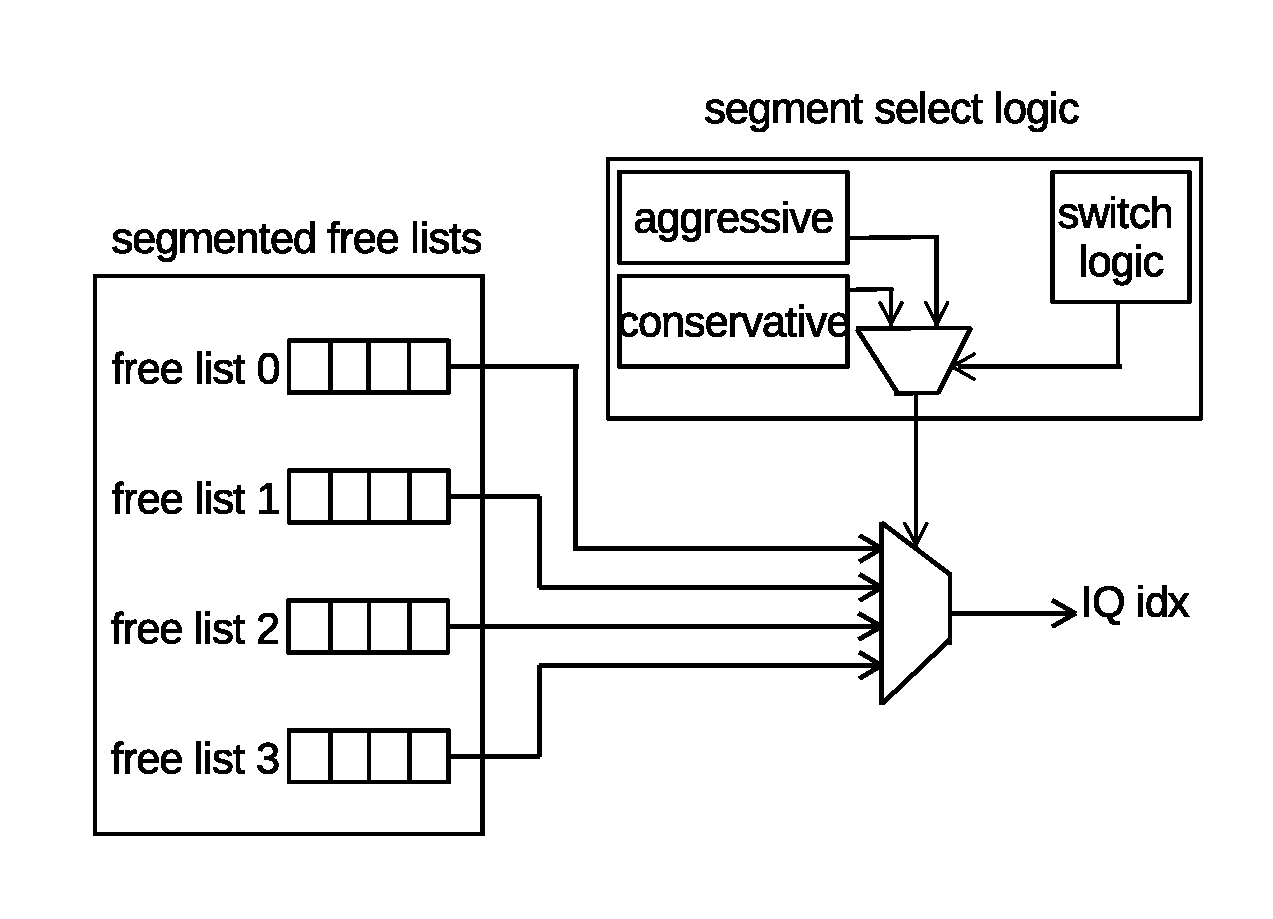
\includegraphics[keepaspectratio, scale=.8]{switch}
  \caption{SWITCH 方式におけるディスパッチエントリの決定回路}
  \label{fig:switch}
\end{figure}

\subsubsection{切り替えアルゴリズム}
切り替えアルゴリズムは以下に示すとおりである.一定のインターバルにおいて,ISR と LLC MPKI を測定し,ILP および MLP の高低を判断する.ILP または MLP のいずれかが高いと判定された場合,次のインターバルを CONSERVATIVE モードで実行する.ILP と MLP がどちらも低いと判定された場合,次のインターバルを AGGRESSIVE モードで実行する.

SWITCH 方式におけるディスパッチするエントリの決定回路を\fig{switch}に示す.AGGRESSIVE と CONSERVATIVE の 2 つの選択アルゴリズムのうち,どちらを利用するかを SWITCH 回路が選択し,その結果に応じてセグメントが選択される.


% 
\chapter{まとめ}
\label{sec:summary}
LSIの微細化の進展に伴って,経年劣化が加速し摩耗故障が増加する問題が深刻になっている.この故障は,デバイスの温度に関して指数関数的に加速するため,チップ内のホット・スポットの解消が求められている.

発行キューはこのホット・スポットの 1 つとして知られている.この主な原因はウェイクアップ時の多数のタグ比較である.本論文では,ウェイクアップ時のタグ比較回数を削減するために,発行キューをセグメント化,および,それに関わるいくつかの手法を提案した.

提案手法には発行キューの容量効率が低下するという問題点が存在する.この問題点に対して,本論文ではさらに,異なる 2 つのディスパッチ・アルゴリズムを,性能についての容量効率の重要性に応じて切り替えて使用することにより,容量効率の低下による性能低下を抑制する手法を提案した.提案手法を SPEC CPU 2017 を使って評価したところ,性能低下を最大でも 5\% 以下に抑えつつ,タグ比較回数を 82\% 削減できることを確認した.



% 付録(必要に応じてコメントを外したり,新たに追加する)
% \appendix
% 
\chapter{SWITCH 方式のしきい値の評価}
\label{sec:appendix1}

\refsec{eval_threshold}で説明したしきい値に関する評価に関して,既に説明した(8,2)以外のセグメント数の組み合わせでの評価結果を示す.評価手順は\refsec{eval_threshold}で説明したものと同様である.なお,ILP の評価値としては ISR と IPC よりも有効であることから,ISR のしきい値の評価に関しては省略し,IPC と LLC MPKI のしきい値の評価のみ説明する.

評価結果を,\fig{4_1_IPC}から\fig{8_4_MPKI}に示す.各図は,IPC 及び  LLC MPKI を変化させた場合の,SWITCH 方式において CONSERVATIVE モードで実行される割合を示している(\fig{switch_IPC_rate}や\fig{switch_MPKI_rate}と同様の形式).

これらの評価をもとに,(8,2)の場合と同様に最適なしきい値を求めた.各セグメント数での最適と判断したしきい値を\tab{switch_threshold_all}に示す.

LLC MPKI に関しては,全ての組み合わせにおいて 2.0 と同一のしきい値となっている.これは,セグメント数が変化しても,LLC MPKI はほとんど変化しないためである.

これに対して, IPC のしきい値はセグメントの総数が 16 までは共通で 3.5 となっているが,セグメントの総数が 32 の組み合わせにおいては,3.0 や 2.5 と最適なしきい値が低下していることがわかる.この理由を説明する.

ILP のしきい値が変化している理由は,cactusBSSN ベンチマークにおいてセグメントの総数が 32 の場合に急激に性能が低下するためである.cactusBSSN は ILP の高いベンチマークの一つで,BASE モデルにおいて IPC が 3.6 程度である.セグメントの総数が 16 以下の場合,このベンチマークは AGGRESSIVE モードにおいても大きな性能低下を起こさないが,セグメントの総数が 32 の場合にはAGGRESSIVE モードで 10\% 以上の大きな性能低下を起こす.その際,IPC は 3.3 程度((16,2)の場合)となる.

この場合に,IPC のしきい値が 3.5 であるような例を考える.このとき,AGGRESSIVE モードでの IPC は 3.3 であるためしきい値を下回り,ILP が低いと判定される.その結果,本来 ILP が高いと評価され CONSERVATIVE モードで実行されるべきであるが,AGGRESSIVE モードで実行され,性能が低下する.実際に,IPC のしきい値が 3.5 の場合には,\fig{16_2_IPC}の cactusBSSN を見るとわかるように CONSERVATIVE モードの割合が低いことがわかる.

このように,セグメントの総数が多い場合には,IPC のしきい値が高い場合に,本来 ILP が高いと判定したいプログラムにおいて,AGGRESSIVE モードでの性能低下が大きく,その結果 ILP が低いと誤って判定されることがある.したがって,セグメントの総数を多くする場合には,IPC のしきい値をある程度低く設定し,ILP の誤った判定を防ぐ必要があると言える.

\begin{table}[tb]
  \caption{セグメント数ごとの SWITCH 方式のしきい値}
  \footnotesize
  \center
    \begin{tabular}{c|c|c|c} \hline \hline
    総セグメント数 & (M-seg,S-seg) & IPC & LLC MPKI \\ \hline
    4 &(4,1) & 3.5 & 2.0 \\
    &(2,2) & 3.5 & 2.0 \\ \hline
    8 &(8,1) & 3.5 & 2.0 \\
    &(4,2) & 3.5 & 2.0 \\ \hline
    &(16,1) & 3.5 & 2.0 \\
    16 &(8,2) & 3.5 & 2.0 \\
    &(4,4) & 3.5 & 2.0 \\ \hline
    &(32,1) & 2.5 & 2.0 \\
    32 &(16,2) & 3.0 & 2.0 \\
    &(8,4) & 3.0 & 2.0 \\ \hline
  \end{tabular}
  \label{tab:switch_threshold_all}
\end{table}

%(4,1)
\begin{figure}[tb]
  \centering
  \includegraphics[keepaspectratio, scale=.8]{4_1_IPC}
  \caption{IPC を用いた SWITCH 方式の制御(4,1)}
  \label{fig:4_1_IPC}

  \centering
  \includegraphics[keepaspectratio, scale=.8]{4_1_MPKI}
  \caption{LLC MPKI を用いた SWITCH 方式の制御(4,1)}
  \label{fig:4_1_MPKI}
\end{figure}

%(2,2)
\begin{figure}[tb]
  \centering
  \includegraphics[keepaspectratio, scale=.8]{2_2_IPC}
  \caption{IPC を用いた SWITCH 方式の制御(2,2)}
  \label{fig:2_2_IPC}

  \centering
  \includegraphics[keepaspectratio, scale=.8]{2_2_MPKI}
  \caption{LLC MPKI を用いた SWITCH 方式の制御(2,2)}
  \label{fig:2_2_MPKI}
\end{figure}

%(8,1)
\begin{figure}[tb]
  \centering
  \includegraphics[keepaspectratio, scale=.8]{8_1_IPC}
  \caption{IPC を用いた SWITCH 方式の制御(8,1)}
  \label{fig:8_1_IPC}

  \centering
  \includegraphics[keepaspectratio, scale=.8]{8_1_MPKI}
  \caption{LLC MPKI を用いた SWITCH 方式の制御(8,1)}
  \label{fig:8_1_MPKI}
\end{figure}

%(4,2)
\begin{figure}[tb]
  \centering
  \includegraphics[keepaspectratio, scale=.8]{4_2_IPC}
  \caption{IPC を用いた SWITCH 方式の制御(4,2)}
  \label{fig:4_2_IPC}

  \centering
  \includegraphics[keepaspectratio, scale=.8]{4_2_MPKI}
  \caption{LLC MPKI を用いた SWITCH 方式の制御(4,2)}
  \label{fig:4_2_MPKI}
\end{figure}

%(16,1)
\begin{figure}[tb]
  \centering
  \includegraphics[keepaspectratio, scale=.8]{16_1_IPC}
  \caption{IPC を用いた SWITCH 方式の制御(16,1)}
  \label{fig:16_1_IPC}

  \centering
  \includegraphics[keepaspectratio, scale=.8]{16_1_MPKI}
  \caption{LLC MPKI を用いた SWITCH 方式の制御(16,1)}
  \label{fig:16_1_MPKI}
\end{figure}

%(4,4)
\begin{figure}[tb]
  \centering
  \includegraphics[keepaspectratio, scale=.8]{4_4_IPC}
  \caption{IPC を用いた SWITCH 方式の制御(4,4)}
  \label{fig:4_4_IPC}

  \centering
  \includegraphics[keepaspectratio, scale=.8]{4_4_MPKI}
  \caption{LLC MPKI を用いた SWITCH 方式の制御(4,4)}
  \label{fig:4_4_MPKI}
\end{figure}

%(32,1)
\begin{figure}[tb]
  \centering
  \includegraphics[keepaspectratio, scale=.8]{32_1_IPC}
  \caption{IPC を用いた SWITCH 方式の制御(32,1)}
  \label{fig:32_1_IPC}

  \centering
  \includegraphics[keepaspectratio, scale=.8]{32_1_MPKI}
  \caption{LLC MPKI を用いた SWITCH 方式の制御(32,1)}
  \label{fig:32_1_MPKI}
\end{figure}

%(16,2)
\begin{figure}[tb]
  \centering
  \includegraphics[keepaspectratio, scale=.8]{16_2_IPC}
  \caption{IPC を用いた SWITCH 方式の制御(16,2)}
  \label{fig:16_2_IPC}

  \centering
  \includegraphics[keepaspectratio, scale=.8]{16_2_MPKI}
  \caption{LLC MPKI を用いた SWITCH 方式の制御(16,2)}
  \label{fig:16_2_MPKI}
\end{figure}

%(8,4)
\begin{figure}[tb]
  \centering
  \includegraphics[keepaspectratio, scale=.8]{8_4_IPC}
  \caption{IPC を用いた SWITCH 方式の制御(8,4)}
  \label{fig:8_4_IPC}

  \centering
  \includegraphics[keepaspectratio, scale=.8]{8_4_MPKI}
  \caption{LLC MPKI を用いた SWITCH 方式の制御(8,4)}
  \label{fig:8_4_MPKI}
\end{figure}


% 発表実績(なければコメントアウトしておく)

\chapter*{発表実績}
\addcontentsline{toc}{chapter}{発表実績}
\noindent
  森健一郎,安藤秀樹,``容量効率を意識したソース・タグ値に基づくセグメント化による発行キューのエネルギー削減,'' 情報処理学会研究報告,Vol.2020-ARC-241,No.3,pp.1-12,2020年7月.

% 謝辞

\chapter*{謝辞}
\addcontentsline{toc}{chapter}{謝辞}
本研究を進めるにあたり,多大なる御指導と御鞭撻を賜わりました名古屋大学大学院工学研究科 情報・通信工学専攻 安藤秀樹教授に心より感謝いたします.また,本研究の遂行を支えてくださいました,名古屋大学大学院工学研究科情報・通信工学専攻安藤研究室の諸氏に深く感謝します.

% ---------- ユーザ入力ここまで ----------


% 参考文献
\bibliographystyle{IEEEtran} 
\bibliography{ref_swopp}

\end{document}
